\chapter{System Overview}
\label{chap:architecture}

% Overview of the main components in the system
% UML diagram, conceptual data model

This chapter will describe the different high-level components in the system and what they do. The main objective of the project was to create an API that enables data gathering from Google Analytics. This made the system API oriented as much of the focus during the project was on the API itself. Although the website could have been implemented as a traditional dynamic website in for example PHP, JSP or ASP.NET \cite{Build81:online}, developing a SPA (Single page application) website using an API-first approach made it possible for team members to specialize within certain technologies applied on different aspects of the system. For further reading on challenges related to this, see Section \ref{sec:furtherImprovements}.

\begin{figure}[h]
  \centering
  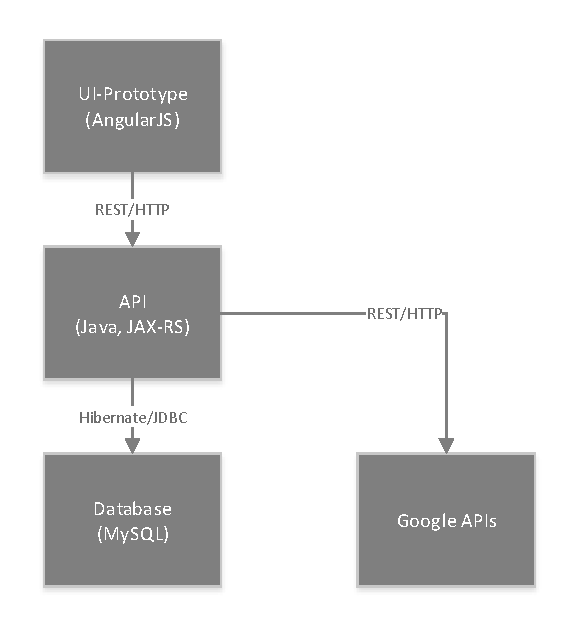
\includegraphics[width=.5\textwidth]{figures/System_overview.pdf}
  \caption[System overview.]{Overview of the system architecture.}
  \label{fig:systemOverview}
\end{figure}

Figure~\ref{fig:systemOverview} gives an overview of the components in the system. How these components are implemented is described in-depth under Chapter~\ref{chap:implementation}. The UI-Prototype is a prototype web application that visualizes what capabilities the API has, it can also be seen as a proof of concept. This application will communicate with the API that is the core of this project. The API will manage data from external Google APIs (Such as Google Analytics Core Reporting API \cite{GoogleAnalyticsCoreAPI} and user data APIs) and store any necessary data in a MySQL database. The data stored in the database could for example be user information, access tokens and information about the different websites a user wants to manage in the system. 